\documentclass[11pt]{scrartcl} 
\PassOptionsToPackage{usenames,dvipsnames,svgnames}{xcolor}  
\usepackage{tikz}
\usetikzlibrary{arrows,positioning,automata}

\begin{document}
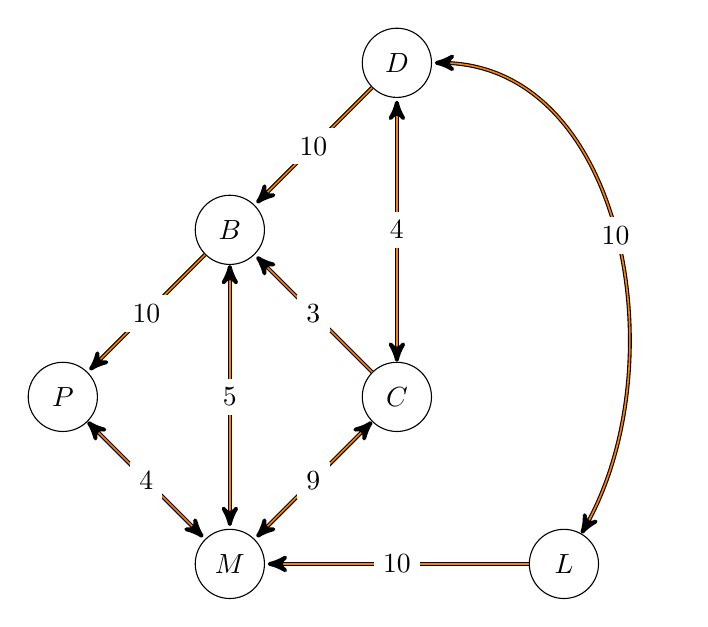
\begin{tikzpicture}[>=stealth',shorten >=1pt,node distance=3cm,on grid,initial/.style    ={}]
  \node[state]          (P)                        {$P$};
  \node[state]          (B) [above right =of P]    {$B$};
  \node[state]          (M) [below right =of P]    {$M$};
  \node[state]          (D) [above right =of B]    {$D$};
  \node[state]          (C) [below right =of B]    {$C$};
  \node[state]          (L) [below right =of C]    {$L$};
\tikzset{mystyle/.style={->,double=orange}} 
\tikzset{every node/.style={fill=white}} 
\path (C)     edge [mystyle]    node   {$3$} (B)
      (D)     edge [mystyle]    node   {$10$} (B) 
      (L)     edge [mystyle]    node   {$10$} (M)
      (B)     edge [mystyle]    node   {$10$} (P);
\tikzset{mystyle/.style={<->,double=orange}}   
\path (P)     edge [mystyle]   node   {$4$} (M)
      (C)     edge [mystyle]   node   {$9$} (M) 
      (C)     edge [mystyle]   node   {$4$} (D)
      (B)     edge [mystyle]   node   {$5$} (M);
\tikzset{mystyle/.style={<->,relative=false,in=0,out=60,double=orange}}
\path (L)     edge [mystyle]   node   {$10$} (D); 
\end{tikzpicture}
\end{document}
